\documentclass[journal,12pt,twocolumn]{IEEEtran}
\usepackage[none]{hyphenat}
\usepackage{graphicx}
\usepackage{listings}
\usepackage[english]{babel}
\usepackage{graphicx}
\usepackage{caption} 
\usepackage{amsmath}
\usepackage{hyperref}
\usepackage{booktabs}
\usepackage{array}
\usepackage{stix}
\usepackage[utf8]{inputenc}

\begin{document}
\title{\textbf{\\circle Assignment}}
\author{kanekal kousar}
\date{october 2022}

\maketitle


\section{Question}
\textbf{\textit{Q(6), C , Section-A, Chapter-8:}If a circle passes through the point (a,b)and cuts the circle {$x^2+y^2=k^2$} orthogonally, then the equation of the locus of its center is.}

\section{Solution}
\raggedright 

\begin{figure}[h!]
\centering
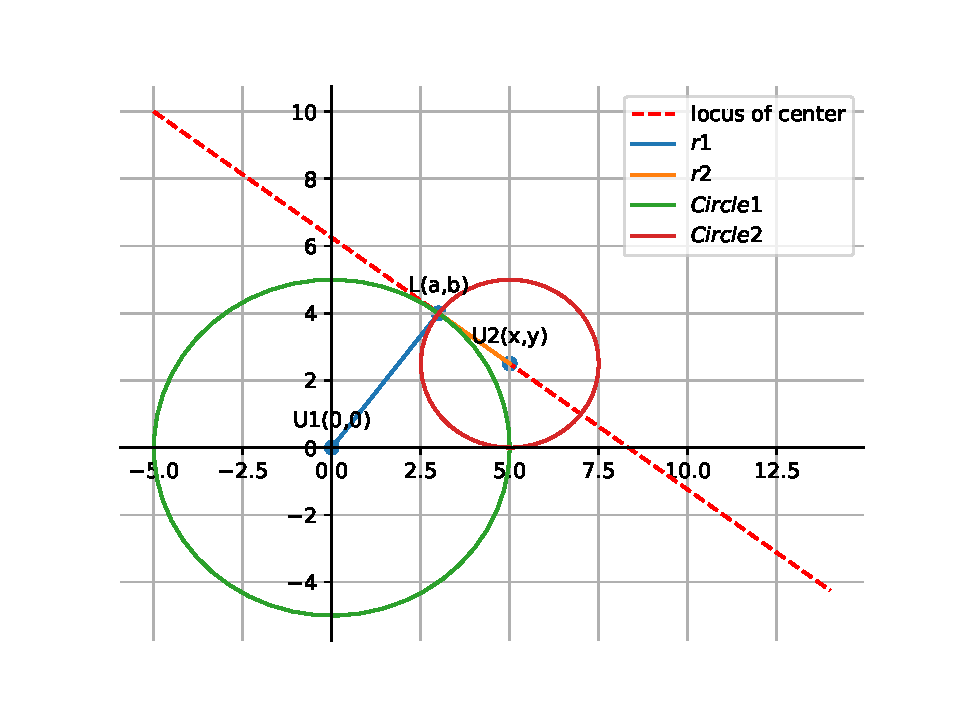
\includegraphics[scale=0.6]{code/cir.pdf}  
\centering
\caption{a circle passes through the point L and cuts the circle {$x^2+y^2=k^2$} orthogonally}
\end{figure}

\vspace{0.25cm}
With the given circle equation {$x^2+y^2=k^2$}, we can find out centre \(U_1\) and radius \(r_1\) of Circle-1
\vspace{0.25cm}
\textbf{STEP-1}

Centre of Circle-1,
\boldmath 
\begin{align} 
\vec{U_1} &= \begin{pmatrix}0 \\ 0 \\ \end{pmatrix} 
\end{align}
\unboldmath

Radius of Circle-1,
\boldmath
\begin{align}
 r_1  &= k
\end{align}
\unboldmath


\textbf{STEP-2}

let,the center of the  circle which passes through the point  L and cuts the circle {$x^2+y^2=k^2$} orthogonally is:
\boldmath 
\begin{align} 
\vec{U_2} = \begin{pmatrix}x \\ y \\ \end{pmatrix}
\end{align} 
\begin{align} 
\vec{L} = \begin{pmatrix}a \\ b \\ \end{pmatrix} 
\end{align}
\unboldmath
Radius of Circle be $r_2$

As both the circles are orthogonal, we get:\vspace{1mm}
\boldmath
\begin{align}
  ||{\vec{U_2} - \vec{U_1}}||^2 &= r_1^2 + r_2^2
\end{align}

where

$\implies||{\vec{U_2}-\vec{U_1}}||^2=||{\vec{U_2}}||^2 + ||{\vec{U_1}}||^2 - 2\vec{U_1}^{\top}\vec{U_2}$

\vspace{0.25cm}
\hspace{3.25cm}=$\vec{U_2}\vec{U_2}^{\top}$
\begin{align}
=\begin{pmatrix}x \\ y \\ \end{pmatrix} \begin{pmatrix}x & y \\ \end{pmatrix} 
\end{align}
\begin{align}
\hspace{-3.25cm}\implies r_1^2=k^2\hspace{3cm}
\end{align}
$\implies r_2^2=||{\vec{U_2}-\vec{L}}||^2$
\begin{align}
\hspace{-1.75cm}=\begin{pmatrix}U_2-L \\ \end{pmatrix} \begin{pmatrix}U_2-L \\ \end{pmatrix}^{\top}
\end{align}

substitute equation (6),(7),(8) in equation (5)
$\implies ||{\vec{U_2} - \vec{U_1}}||^2 = r_1^2 + r_2^2$
\hspace{1cm}$\implies \begin{pmatrix}x \\ y \\ \end{pmatrix} \begin{pmatrix}x & y \\ \end{pmatrix}=k^2+
\begin{pmatrix}U_2-L \\ \end{pmatrix} \begin{pmatrix}U_2-L \\ \end{pmatrix}^{\top}$
\unboldmath
by solving the above equation we get,
\boldmath
$\implies x^2+y^2 = x^2+a^2-2ax+y^2+b^2by+k^2$

$\implies a^2+b^2+k^2-2ax-2by=0$
\begin{align}
\hspace{-2cm}\implies 2ax+2by-(a^2+b^2+k^2)=0
\end{align}
\unboldmath 

equation (9) is the required equation
\section*{Construction}
\centering
\vspace{0.2cm}
{
\setlength\extrarowheight{2pt}
\begin{tabular}{|c|c|c|}
	\hline
	\textbf{Symbol}&\textbf{Value}&\textbf{Description}\\
	\hline
	$\vec{U_1}$ & $\begin{pmatrix}0 \\ 0 \\ \end{pmatrix}$ & center of given circle\\
	\hline
	$r_1$ & k & radius of given circle\\
	\hline
	$\vec{U_2}$ & $\begin{pmatrix}x \\ y \\ \end{pmatrix}$ & center of circle 2\\
	\hline
	$\vec{L}$ & $\begin{pmatrix}a \\ b \\ \end{pmatrix}$ & a point on  circle 2\\
	\hline
	$r_2$ & $||{\vec{U_2}-\vec{L}}||^2$ & radius of circle 2\\
	\hline
\end{tabular}
}

\vspace{0.6cm}
Get the python code of the figures from
\begin{table}[h]
\large
\centering
\framebox{
\url{https://github.com/kkousar/KOUSAR_FWC/blob/main/circle_Assignment/code/circle.py}}
\bibliographystyle{ieeetr}

\end{table}



\end{document}
